% Options for packages loaded elsewhere
\PassOptionsToPackage{unicode}{hyperref}
\PassOptionsToPackage{hyphens}{url}
%
\documentclass[
  12pt,
]{article}
\usepackage{lmodern}
\usepackage{amssymb,amsmath}
\usepackage{ifxetex,ifluatex}
\ifnum 0\ifxetex 1\fi\ifluatex 1\fi=0 % if pdftex
  \usepackage[T1]{fontenc}
  \usepackage[utf8]{inputenc}
  \usepackage{textcomp} % provide euro and other symbols
\else % if luatex or xetex
  \usepackage{unicode-math}
  \defaultfontfeatures{Scale=MatchLowercase}
  \defaultfontfeatures[\rmfamily]{Ligatures=TeX,Scale=1}
\fi
% Use upquote if available, for straight quotes in verbatim environments
\IfFileExists{upquote.sty}{\usepackage{upquote}}{}
\IfFileExists{microtype.sty}{% use microtype if available
  \usepackage[]{microtype}
  \UseMicrotypeSet[protrusion]{basicmath} % disable protrusion for tt fonts
}{}
\makeatletter
\@ifundefined{KOMAClassName}{% if non-KOMA class
  \IfFileExists{parskip.sty}{%
    \usepackage{parskip}
  }{% else
    \setlength{\parindent}{0pt}
    \setlength{\parskip}{6pt plus 2pt minus 1pt}}
}{% if KOMA class
  \KOMAoptions{parskip=half}}
\makeatother
\usepackage{xcolor}
\IfFileExists{xurl.sty}{\usepackage{xurl}}{} % add URL line breaks if available
\IfFileExists{bookmark.sty}{\usepackage{bookmark}}{\usepackage{hyperref}}
\hypersetup{
  pdftitle={Black Lives Matter Protests and Voter Turnout},
  pdfauthor={Cameron Kimble; Kevin Morris; Kasey Zapatka\^{}{[}XX\}},
  hidelinks,
  pdfcreator={LaTeX via pandoc}}
\urlstyle{same} % disable monospaced font for URLs
\usepackage[margin=1in]{geometry}
\usepackage{longtable,booktabs}
% Correct order of tables after \paragraph or \subparagraph
\usepackage{etoolbox}
\makeatletter
\patchcmd\longtable{\par}{\if@noskipsec\mbox{}\fi\par}{}{}
\makeatother
% Allow footnotes in longtable head/foot
\IfFileExists{footnotehyper.sty}{\usepackage{footnotehyper}}{\usepackage{footnote}}
\makesavenoteenv{longtable}
\usepackage{graphicx}
\makeatletter
\def\maxwidth{\ifdim\Gin@nat@width>\linewidth\linewidth\else\Gin@nat@width\fi}
\def\maxheight{\ifdim\Gin@nat@height>\textheight\textheight\else\Gin@nat@height\fi}
\makeatother
% Scale images if necessary, so that they will not overflow the page
% margins by default, and it is still possible to overwrite the defaults
% using explicit options in \includegraphics[width, height, ...]{}
\setkeys{Gin}{width=\maxwidth,height=\maxheight,keepaspectratio}
% Set default figure placement to htbp
\makeatletter
\def\fps@figure{htbp}
\makeatother
\setlength{\emergencystretch}{3em} % prevent overfull lines
\providecommand{\tightlist}{%
  \setlength{\itemsep}{0pt}\setlength{\parskip}{0pt}}
\setcounter{secnumdepth}{5}
\usepackage{rotating}
\usepackage{setspace}
\usepackage{booktabs}
\usepackage{longtable}
\usepackage{array}
\usepackage{multirow}
\usepackage{wrapfig}
\usepackage{float}
\usepackage{colortbl}
\usepackage{pdflscape}
\usepackage{tabu}
\usepackage{threeparttable}
\usepackage{threeparttablex}
\usepackage[normalem]{ulem}
\usepackage{makecell}
\usepackage{xcolor}
\newlength{\cslhangindent}
\setlength{\cslhangindent}{1.5em}
\newenvironment{cslreferences}%
  {\setlength{\parindent}{0pt}%
  \everypar{\setlength{\hangindent}{\cslhangindent}}\ignorespaces}%
  {\par}

\title{Black Lives Matter Protests and Voter Turnout\thanks{The authors thank XX for their feedback and support. All errors are our responsibility.}}
\author{Cameron Kimble\footnote{XX} \and Kevin Morris\footnote{XX} \and Kasey Zapatka\^{}{[}XX\}}
\date{January 21, 2021}

\begin{document}
\maketitle
\begin{abstract}
This is an abstract.
\end{abstract}

\pagenumbering{gobble}
\pagebreak

\pagenumbering{arabic}
\begin{center}
Black Lives Matter Protests and Voter Turnout
Cameron Kimble, Kevin Morris, and Kasey Zapatka
\end{center}

\hypertarget{introduction}{%
\subsubsection*{Introduction}\label{introduction}}
\addcontentsline{toc}{subsubsection}{Introduction}

TKTKTKTK
Political socialization, in recent years, is more and more defined as the gradual development of an individual's political preferences, and more broadly, their perceptions of the political world -- the norms and behaviors internalized within a given society (Fillieule \protect\hyperlink{ref-Fillieule2013}{2013}). However, socialization research in the past has focused on why people do or do not participate in politics, as opposed to the socialization effects of participation in explicitly political organizations.
Given the resurgence of mass protest, we seek to understand the socializing effects of participation in social movements (or protest movements). Prior research (Snow et al. \protect\hyperlink{ref-Snow1986}{1986}) indicates that initial frame alignment (``schemata of interpretation'') between an individual and a social movement organization is a precondition of participation, and that frame alignment is a continuing process that occurs between individuals and social movements, transforming and reinforcing the individual's ideological orientations.
Research on American activists in the 1960s has addressed the effects of participation on a social movement on political behaviors and views. Indeed, one study found that participating in the Freedom Summer project caused volunteers to become ``radicalized,'' and were thus significantly more likely to participate in social movements in subsequent years (McAdam \protect\hyperlink{ref-McAdam1989}{1989}). In a similar study, researchers conclude that involvement with social movements through the 1960s and 1970s caused participants to become significantly more liberal in political orientation, as evidenced by subsequent political engagement -- voting for Jimmy Carter, and participating in subsequent demonstrations (Sherkat and Blocker \protect\hyperlink{ref-Sherkat1997}{1997}).
Harnessing discontent, and channeling it into political/social movement
-Rustin
Raising awareness/developing critical conscious through Social movement participation

\hypertarget{literature-on-protests-and-mobilization}{%
\subsubsection*{Literature on Protests and Mobilization}\label{literature-on-protests-and-mobilization}}
\addcontentsline{toc}{subsubsection}{Literature on Protests and Mobilization}

Cameron to fill

\hypertarget{the-mobilizing-potential-of-injustice-narratives}{%
\subsubsection*{The Mobilizing Potential of Injustice Narratives}\label{the-mobilizing-potential-of-injustice-narratives}}
\addcontentsline{toc}{subsubsection}{The Mobilizing Potential of Injustice Narratives}

Although protests can be a site of key political socialization, the Black Lives Matter movement centers on a social issue that has historically been \emph{demobilizing.} Much research over the past decade has demonstrated that contact with the legal system causes individuals to withdraw from political socialization (see, for instance, Lerman and Weaver \protect\hyperlink{ref-Lerman2014}{2014}). These demobilizing effects may extend even to individuals who have \emph{not} been formally convicted, but rather are in close contact with those who have been (Morris \protect\hyperlink{ref-Morris2020}{2020}; but see {\textbf{???}}). The relationship, however, is complicated: Walker (\protect\hyperlink{ref-Walker2014}{2014}) shows that individuals in ``proximal contact'' --- whose family members have been convicted --- become more likely to participate in non-electoral political activities.

Walker (\protect\hyperlink{ref-Walker2020}{2020}), however, provides key insight into how the generally demobilizing effects of contact with the legal system can be transformed into a \emph{mobilizing} force. Walker argues that, when individuals locate their experience with the legal system in narratives of (racial) injustice, the contact can cause them to take action. The Black Lives Matter movement aimed to do just this. BLM activists called attention to the fact that American police forces have a long history of racially discriminatory practices. The widespread protests may have caused individuals in close contact with police and the legal system to understand their contact with the police and legal systems \emph{not} as personal failings but as a key producer of racial inequity. The recent work from Hannah Walker indicates that this may have been a mobilizing event.

\hypertarget{data-and-methods}{%
\subsubsection*{Data and Methods}\label{data-and-methods}}
\addcontentsline{toc}{subsubsection}{Data and Methods}

To understand the relationship between protests and turnout, we leverage two primary datasets. First, we employ data collected by the US Crisis Monitor\footnote{See \url{https://acleddata.com/download/22846/}.} which records the location of every Black Lives Matter protest during 2020. These events are geocoded, which allow us to identify the precise location of each protest.

Our second primary data source is the national, geocoded voter file made available by L2 Political. The voter file includes a host of information about every registered voter in the country, including their gender, age, partisan affiliation, and race (L2 models the characteristics that are not reported in each state's public voter file). The registered voter file also includes historical voter turnout for both the 2020 and historical elections. At this point, not all states have yet entered their 2020 voter turnout into the registered voter file.

We intend to measure whether how far a voter lived from a Black Lives Matter protest in the summer of 2020 was correlated with their turnout in November. Using these geocoded records, we measure the distance between each voter and the closest protest, and test whether this distance is significantly related to turnout after controlling for other relevant characteristics, \emph{including} past turnout.

To be sure, this cannot prove the causal link between exposure to protest and increased turnout. Voters were not ``randomly'' exposed to protests; the same factors that primed an area to stage a protest may have also primed them to turn out at higher rates in the 2020 election. To identify the causal effect of exposure to protest on voter turnout we therefore leverage variation in rainfall (relative to historical rainfall) in the week following the murder of George Floyd in an instrumental variable framework. We expect that areas with higher rainfall likely had fewer protests, \emph{regardless} of whether that area was likely to turn out at high rates in November. For a fuller discussion of how rainfall can be used to instrument exposure to political protests, see Madestam et al. (\protect\hyperlink{ref-Madestam2013}{2013}).

\hypertarget{preliminary-results}{%
\subsubsection*{Preliminary Results}\label{preliminary-results}}
\addcontentsline{toc}{subsubsection}{Preliminary Results}

As mentioned above, individual-level turnout records are not yet widely available, but will be published in the first half of 2021. The records are available, however, for the states of Georgia and North Carolina which we use as pilot studies.

Figure \ref{fig:map} displays the location of all protests staged in June, 2020, in Georgia and North Carolina. We also show the distribution of voters around the state.

\begin{figure}[H]
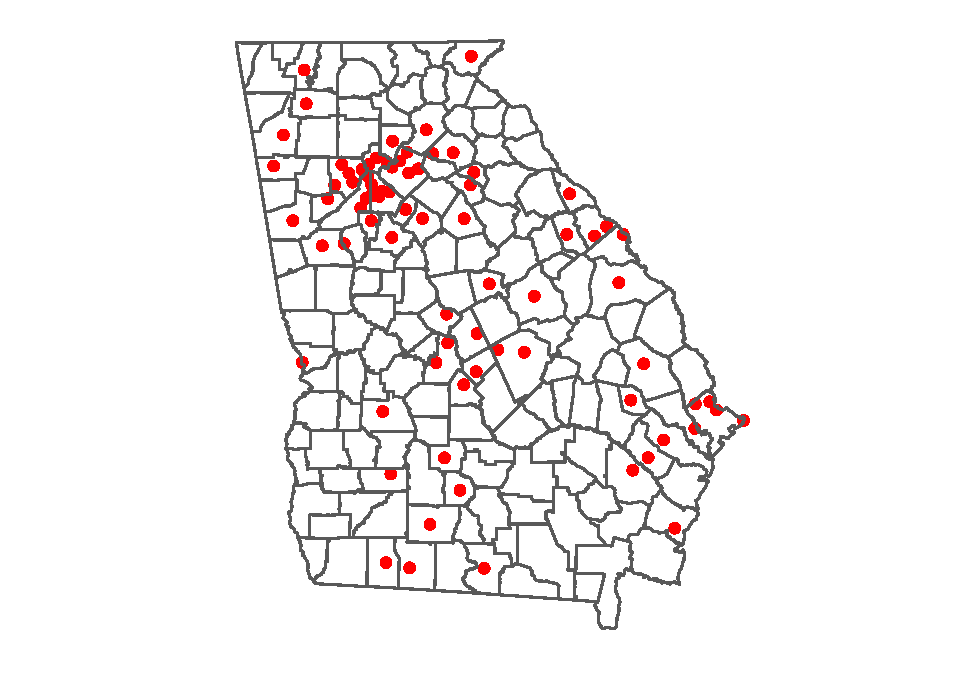
\includegraphics[width=0.5\linewidth]{asa_abstract_files/figure-latex/figures-side-1} 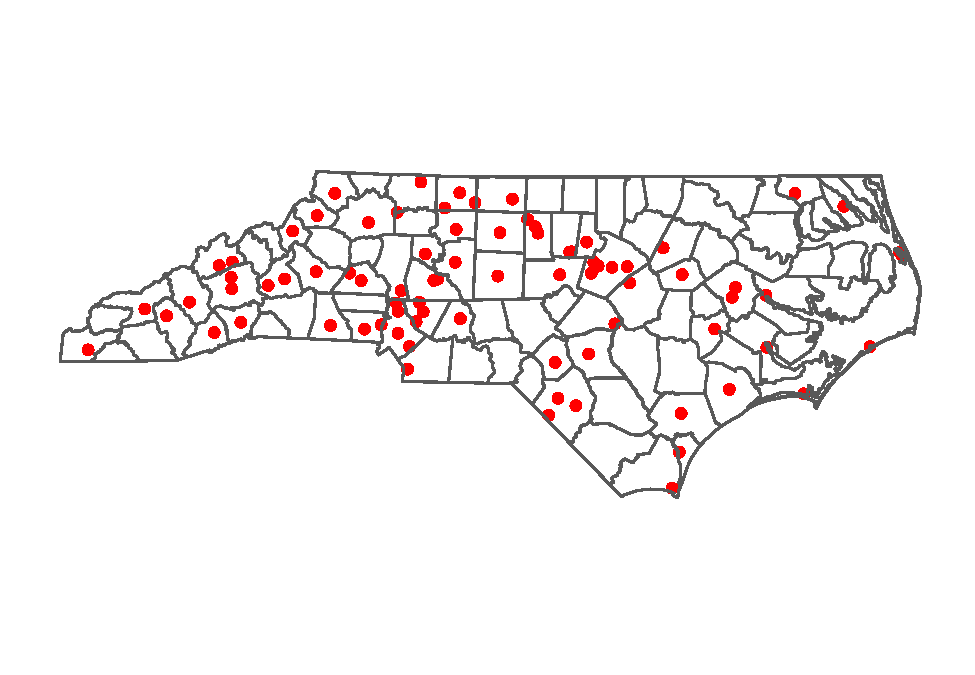
\includegraphics[width=0.5\linewidth]{asa_abstract_files/figure-latex/figures-side-2} \caption{\label{fig:map}Sites of June, 2020, Protests}\label{fig:figures-side}
\end{figure}

In Table \ref{tab:reg} we present the results of an ordinary least-squares regression, where each observation is a registered voter. The dependent variable \emph{Voted in 2020} measures whether a voter participated in the 2020 general election, and the primary dependent variable \emph{Distance} measures how far the voter lived from the nearest June protest in their state. We also control for other individual- and neighborhood-level characteristics, including each voter's own participation history. Robust standard errors are clustered by county.\footnote{These are currently run on random 10 percent samples, stratified by county, due to computing restraints. The models will be run on the full universe of voters in the full paper.}

\begin{singlespace}
\input{"../temp/big_reg_formatted.tex"}
\end{singlespace}

\hypertarget{what-comes-next}{%
\subsubsection*{What Comes Next}\label{what-comes-next}}
\addcontentsline{toc}{subsubsection}{What Comes Next}

Our results from Georgia indicate that the relationship between distance to protests and turnout is more complicated than we initially expected. This is perhaps true for both methodological reasons and for theoretical ones. Methodologically, we have not yet implemented the IV model which will allow us to more precisely estimate the causal effect of protest exposure. Moreover, Figure \ref{fig:map} demonstrates that there is clear spatial patterning in the siting of protests; we need to implement spatial regression models to fully account for this. Theoretically, it may be that exposure to protest has different effects on different voters, and that a single estimate of exposure is muddying heterogeneous effects; our full paper will explore this potentiality.

\newpage

\hypertarget{references}{%
\subsubsection*{References}\label{references}}
\addcontentsline{toc}{subsubsection}{References}

\hypertarget{refs}{}
\begin{cslreferences}
\leavevmode\hypertarget{ref-Fillieule2013}{}%
Fillieule, Olivier. 2013. ``Political Socialization and Social Movements.'' In \emph{The Wiley-Blackwell Encyclopedia of Social and Political Movements}. American Cancer Society. \url{https://doi.org/10.1002/9780470674871.wbespm199}.

\leavevmode\hypertarget{ref-Lerman2014}{}%
Lerman, Amy E., and Vesla M. Weaver. 2014. \emph{Arresting Citizenship: The Democratic Consequences of American Crime Control}. Chicago Studies in American Politics. Chicago ; London: The University of Chicago Press.

\leavevmode\hypertarget{ref-Madestam2013}{}%
Madestam, Andreas, Daniel Shoag, Stan Veuger, and David Yanagizawa-Drott. 2013. ``Do Political Protests Matter? Evidence from the Tea Party Movement*.'' \emph{The Quarterly Journal of Economics} 128 (4): 1633--85. \url{https://doi.org/10.1093/qje/qjt021}.

\leavevmode\hypertarget{ref-McAdam1989}{}%
McAdam, Doug. 1989. ``The Biographical Consequences of Activism.'' \emph{American Sociological Review} 54 (5): 744--60. \url{https://doi.org/10.2307/2117751}.

\leavevmode\hypertarget{ref-Morris2020}{}%
Morris, Kevin. 2020. ``Neighborhoods and Felony Disenfranchisement: The Case of New York City.'' \emph{Urban Affairs Review}, May, 1078087420921522. \url{https://doi.org/10.1177/1078087420921522}.

\leavevmode\hypertarget{ref-Sherkat1997}{}%
Sherkat, Darren E., and T. Jean Blocker. 1997. ``Explaining the Political and Personal Consequences of Protest.'' \emph{Social Forces} 75 (3): 1049--70. \url{https://doi.org/10.2307/2580530}.

\leavevmode\hypertarget{ref-Snow1986}{}%
Snow, David A., E. Burke Rochford, Steven K. Worden, and Robert D. Benford. 1986. ``Frame Alignment Processes, Micromobilization, and Movement Participation.'' \emph{American Sociological Review} 51 (4): 464--81. \url{https://doi.org/10.2307/2095581}.

\leavevmode\hypertarget{ref-Walker2014}{}%
Walker, Hannah L. 2014. ``Extending the Effects of the Carceral State: Proximal Contact, Political Participation, and Race.'' \emph{Political Research Quarterly}, July. \url{https://doi.org/10.1177/1065912914542522}.

\leavevmode\hypertarget{ref-Walker2020}{}%
---------. 2020. ``Targeted: The Mobilizing Effect of Perceptions of Unfair Policing Practices.'' \emph{The Journal of Politics} 82 (1): 119--34. \url{https://doi.org/10.1086/705684}.
\end{cslreferences}

\end{document}
